\documentclass{article}
\usepackage{tikz}
\usepackage{caption}
\usepackage{listings}
\usepackage{xcolor}
\usepackage{multicol}
\usepackage{geometry}
\lstset { %
    language=Python,
    backgroundcolor=\color{black!5}, % set backgroundcolor
    basicstyle=\footnotesize,% basic font setting
}
\usetikzlibrary{shapes}
\geometry{
  left={1cm},
  right={1cm}
}

\author{Asher Griess, David Medin}
\title{R Tree Algorithm}
\begin{document}
\maketitle


\begin{multicols}{2}[]
\section{Abstract}
\paragraph{}
A R Tree is a data structure used to make spacial computation and comparison much faster than brute force.
The R-tree is very similar to the B-tree in structure, and Quad-Tree in use. One of the main differences is that
R-trees are page-able. This means that they could be put into storage, which could be ideal for very large data sets 
that can't be stored in ram.  You can also take out parts of the R-tree into ram while working with it. A good example
of a program that could use R-trees is a mapping system of the world, where the large data set would be hard to store in memory.
The R-tree is also very good for nearest neighbor searching. Also R-tree can be used to store any type of shape which allow for shapes
of things such as buildings to be put in the minimum bounding rectangle. R-trees have also been used a lot in databases for spacial data.

\section{Basics}

\paragraph{}
A R Tree is parameterized by one variable, $M$, which specifies the maximum number of entries each node is allowed to have. An entry of a node is either a reference
to another node, or a data object. In our implementation, all data objects are points in space.
Based on $M$, is $m = \lceil\frac{M}{2}\rceil$, the minimum number of entries each node must have. A reasonable value for $M$ is 50. \cite{guttman_1984_rtrees} Each entry of a node must have an Minimum Bounding Rectangle,
or MBR (which is also an AABB). This is a rectangle that tightly encloses all of its contents. If an entry to a node is another node which are all parents, then the entry
of the first node will have an MBR encompassing all of its child nodes. Similarly, entries that point to leaf nodes have an MBR encompassing all of the data objects - or points - that belong to that leaf node.

\section{Inserting}
Complexity

average : none

worst case : $O(n)$

When splitting we are trying to find the best leaf node
that will have least increase to the minimum bounding rectangle that it is inserted in.
It should also be noted that when we are at $M$ entries at the inserted leaf node, we
need to split.

\begin{minipage}{\linewidth}
\captionof{figure}{R-Tree Example}
\centering
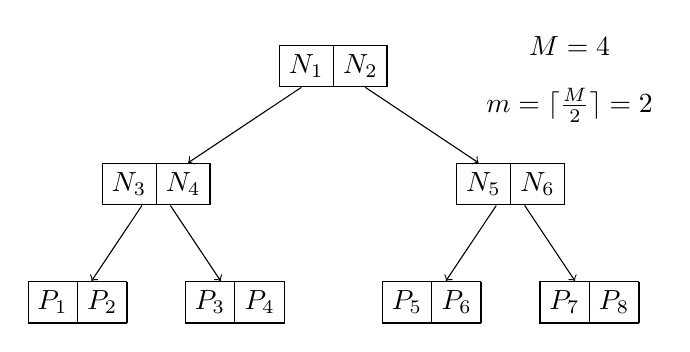
\begin{tikzpicture}
  \draw (3cm,0.25cm) node{$M = 4$};
  \draw (3cm,-0.5cm) node{$m= \lceil\frac{M}{2}\rceil = 2$};
  \tikzstyle{rtree}=[rectangle split, rectangle split horizontal,rectangle split ignore empty parts,draw]
  \tikzstyle{every node}=[rtree]
  \tikzstyle{level 1}=[sibling distance=45mm]
  \tikzstyle{level 2}=[sibling distance=20mm]
  \node {$N_1$ \nodepart{two} $N_2$} [->]
      child {node {$N_3$ \nodepart{two} $N_4$}
      child {node {$P_1$ \nodepart{two} $P_2$}}
      child {node {$P_3$ \nodepart{two} $P_4$}}    
  } 
  child {node {$N_5$ \nodepart{two} $N_6$}
      child {node {$P_5$ \nodepart{two} $P_6$}}
      child {node {$P_7$ \nodepart{two} $P_8$}} 
};
\end{tikzpicture}

Note: In this example the leaf nodes contain the actual points or shapes($P_n$).
\end{minipage}

\subsection*{Pseudo Code}

\begin{lstlisting}    
If at leaf:
  Insert(Entry)
  If(entries > M):
    Split()
  CurrentNode.entries.Add(Entry)
  return
For(each child):
  If(ChildNode.IsEngulf(Entry)):
    Insert(Node)
  else:
    For(each child):
      Find difference in area if Entry were inserted
    insert(NodeWithSmallestDifference);
\end{lstlisting}


\section{Splitting} 
\begin{lstlisting}
# Find Two Points with most extreme distances
BiggestDiff = 0;
For(child i for each child):
  For(child z for each Child):
    BiggestXDiff = max(
      i.box.bottomleft.x-z.box.topleft.x,
      i.box.topleft.x-z.box.bottomleft.x
    );
    BiggestYDiff = max(
      i.box.bottomleft.y-z.box.topleft.y,
      i.box.topleft.y-z.box.bottomleft.y
    );
    if(BiggestXDiff > BiggestDiff)
    {
        BiggestDiff = BiggestXDiff
    }
    if(BiggestYDiff > BiggestDiff)
    {
        BiggestDiff = BiggestYDiff
    }
#Make two nodes with the found extreme boxes
Node newnode1 = new Node()
Node newnode2 = new Node()

#Remove from children
Parent.Remove(box1)
Parent.Remove(box2)

#Take children from old node and put them in new ones
\end{lstlisting}

\section{Searching}

\paragraph{}
The next operation to do on an R Tree is a search for an object. Given an object, the R Tree will search itself for
an object that is equal to the object and return the node that contains it. Searching an R Tree has an average complexity
of $O(log_Mn)$, and a worst case of $O(n)$, making it better, on average, as you increase $M$, the maximum number of entries
per node.

\paragraph{}The first obvious thing to check is whether the root
node's MBR contains the object. If it doesn't, then there is no way it is contained by any of its children and we can stop here.
If it is contained, then we check each of its children and do the same thing, checking for whether the object is totally contained.
For each child that does contain the object, we'll recurse down and start the process over again until we reach a leaf node that
can totally contain the object's MBR inside its MBR. Then, we compare each leaf node entry with the object. If any are equal, then
we have found the leaf node to return from the search.

\section{Removing}

\paragraph{}
When removing a point - or an object - from a R Tree, the first step is to find the leaf node that stores the point.
However, we have already covered that in the previous section, Searching. Now that we have the leaf node that contains
the point, we now remove the point from the leaf node. This may reduce the number of entries this leaf node has to be below
$m$, which is not allowed for nodes that are not root. If the leaf node is the root then we ignore this problem, because
we can't have a smaller tree.\\

\begin{minipage}{\columnwidth}
\captionof{figure}{A snapshot of the bottom of an R Tree. $N_{parent}$ represents the rest of the tree, and $P_n$ represents the data objects.}
\centering
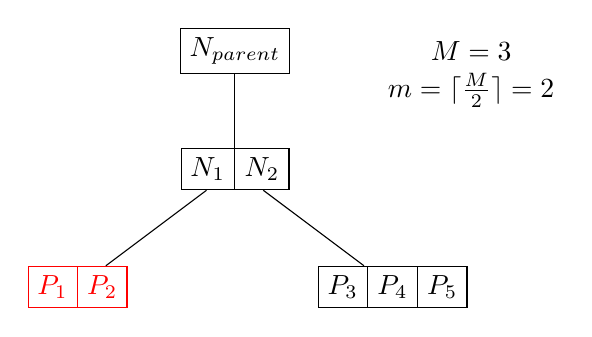
\begin{tikzpicture}
  \draw (3cm,0) node{$M=3$};
  \draw (3cm,-0.5cm) node{$m= \lceil\frac{M}{2}\rceil = 2$};
  \tikzstyle{rtree}=[rectangle split, rectangle split horizontal,rectangle split ignore empty parts,draw]
    \tikzstyle{every node}=[rtree]
    \tikzstyle{level 1}=[sibling distance=45mm]
    \tikzstyle{level 2}=[sibling distance=40mm]
    \node{$N_{parent}$}
    child {node{$N_1$ \nodepart{two} $N_2$}
      child{node[color=red]{$P_1$ \nodepart{two} $P_2$} }
      child{node{$P_3$ \nodepart{two} $P_4$ \nodepart{three} $P_5$}}
    };
\end{tikzpicture}
\label{fig:removing}
\end{minipage}

\paragraph{}
In Figure \ref{fig:removing}, we see that the leaf node $N_1$, which has two entries, is going to have an entry removed. Because $m=3$, the red leaf node will be deleted and its other entry will be reinserted later.After that, because $N_{parent}$ has only one entry, it will be deleted, and we'll recurse through its children and find the three entries is $N_2$ and store those for reinsertion as well.
\paragraph{}
If this node is not the root and has less than $m$ entries, then it is necessary to delete that node. But we don't want to destroy
the other $m - 1$ entries, so we'll store each of the node's entries into a list, or other container type, to insert back into
the tree when we are done removing. Because we are removing the leaf node, this means that its parent's entries can also fall below
$m$ nodes, which then requires that it is deleted too. In that case, a recursive search of all of that parent's children is necessary
to find all points - or other data objects - to store for reinsertion later.
\paragraph{}
Even though it seems that a the leaf node case and the parent node case seem different, they are actually the same case. Parents have
other nodes as their entries and leaf nodes have objects as their entries. Both must have $m \le n \le M$ entries (where $n$ is the number
of entries the node has), and both need to be deleted from their parent and recursively store all of the entries below it in the tree.

\bibliographystyle{plain}
\bibliography{rtree.bib}

\end{multicols}

\end{document}